\documentclass[11pt,a4paper]{article}
\usepackage[margin=2.3cm]{geometry}
\usepackage{amsmath,amssymb,bm}
\usepackage{siunitx}
\usepackage{booktabs}
\usepackage{graphicx}
\usepackage{tikz}
\usetikzlibrary{arrows.meta,calc}
\usepackage{enumitem}
\usepackage{float}
\usetikzlibrary{positioning}
\tikzset{capt/.style={text width=5.2cm,align=center}}
\usepackage[colorlinks=true,linkcolor=blue!60!black,urlcolor=blue!60!black]{hyperref}
\usepackage{fancyhdr}
\usepackage{tcolorbox}
\tcbuselibrary{skins,breakable}
\sisetup{per-mode=symbol,detect-all}

\newtcolorbox{keybox}[1]{colback=blue!4,colframe=blue!50!black,title=#1,fonttitle=\bfseries,breakable}
\newtcolorbox{examplebox}[1]{colback=green!4,colframe=green!40!black,title=#1,fonttitle=\bfseries,breakable}
\newtcolorbox{aerobox}[1]{colback=orange!5,colframe=orange!60!black,title=#1,fonttitle=\bfseries,breakable}

\pagestyle{fancy}
\fancyhf{}
\lhead{
\includegraphics[height=0.6cm]{logos/itu_logo_laci.pdf}\ \ UCK 364E Design of Machine Elements}
\setlength{\headheight}{20pt}
\rhead{Week 1 -- Lecture Notes}
\cfoot{\thepage}

\title{\textbf{UCK 364E Design of Machine Elements}\\[4pt]
\Large Week 1: Mechanical Design in the Aerospace Context\\[2pt]
\large Design factors, factor of safety, fitting factor, and stress--strain review}
\author{Prof.\ Dr.\ Onur Tunçer\\ Department of Aeronautical Engineering, Istanbul Technical University}
\date{Fall 2026}

\begin{document}
\maketitle

\section*{Learning objectives}
By the end of this week you should be able to
\begin{enumerate}[nosep]
  \item explain what a \emph{machine element} is and locate the elements treated in this course on an aircraft;
  \item distinguish limit load, ultimate load, factor of safety, fitting factor and margin of safety, and apply them as the airworthiness codes require;
  \item explain the difference between the ``machine design'' notion of a factor of safety and the regulated aerospace factors;
  \item use A-, B- and S-basis design allowables correctly;
  \item recover the stress--strain tools needed for the rest of the course: 3-D stress state, principal stresses, von Mises and Tresca criteria, stress concentration factors and the basic beam, shaft and pressure-vessel formulae;
  \item choose between the main aerospace alloy families for an element and state the corrosion, temperature and direction caveats that go with each;
  \item write the element-specific notes on a detail drawing---fits, GD\&T, finish, standard parts---and read an ISO 286 fit;
  \item read a bolt or nut standard callout (NAS, MS, EN, ISO) and say what it promises;
  \item recognise ten recurring design errors and their corrections.
\end{enumerate}

\section{What is a machine element, and why a separate course for aeronautical engineers?}

A \emph{machine element} is a standardised load-carrying component that appears again and again in mechanical systems and for which a body of design rules, standards and catalogue data exists: threaded fasteners, rivets, welds, bonded joints, keys and splines, springs, bearings, shafts and gears. The aircraft designer rarely invents a new machine element, but continuously \emph{selects, sizes and integrates} existing ones. Almost every structural failure in service is a failure of an element or of a joint between elements, not of a bulk panel.

The classical machine elements course is organised around rotating machinery: static failure, then fatigue, then shafts, gears, bearings, clutches and brakes. An aircraft inverts the priorities. Table~\ref{tab:where} shows where the elements of this course live on an airframe; note that fatigue and joints dominate, whereas gears are confined to gearboxes and actuators.

\begin{table}[h]
\centering\footnotesize
\begin{tabular}{@{}lp{5.2cm}p{5cm}@{}}
\toprule
Element & Typical aircraft location & Governing concern \\
\midrule
Bolts, Hi-Loks, rivets & Wing--fuselage fittings, lap joints, frames & Fatigue, preload retention, bearing/bypass \\
Lugs and fittings & Wing root, landing-gear trunnion, engine mount & Fitting factor, fatigue, fretting \\
Welds & Steel-tube fuselages, engine mounts, exhaust & Weld fatigue class, NDT \\
Adhesive bonds & Sandwich panels, doublers, repairs, spacecraft & Peel, environment, outgassing \\
Splines, keys, fits & Accessory drives, actuator outputs & Fretting, tolerance stack-up \\
Springs & Landing gear, valves, latches, control feel & Fatigue, surge, relaxation \\
Rolling bearings & Wheels, control-surface hinges, actuators, gearboxes & $L_{10}$ life, load spectrum, lubrication \\
Gears & Accessory gearbox, rotorcraft transmission, flap drive & Tooth bending/contact fatigue \\
\bottomrule
\end{tabular}
\caption{Where the machine elements of this course appear on an aircraft.}
\label{tab:where}
\end{table}

For this reason the course is ordered ``fatigue first'': weeks 2--4 build the fatigue and fracture toolkit and every later element is analysed under cyclic loading from its first appearance.

\section{The design problem: loads, allowables and margin}

Every element design reduces to the comparison
\begin{equation}
  \text{applied stress (or load)} \times \text{factors} \;\le\; \text{allowable stress (or load)}.
\end{equation}
The whole art lies in defining the three ingredients on the right and left correctly.

\subsection{Limit and ultimate load}

A word on the alphabet first. \textbf{CS} stands for \emph{Certification Specifications}, the airworthiness codes published by EASA (the European Union Aviation Safety Agency): CS-25 for large aeroplanes, CS-23 for small aeroplanes, CS-27 and CS-29 for rotorcraft, CS-E for engines. Each CS has a Book 1 containing the binding requirements and a Book 2 containing the \emph{Acceptable Means of Compliance} (AMC), i.e.\ guidance on how to show that a requirement is met. The American counterpart is the \textbf{FAR}, the Federal Aviation Regulations (formally Title 14 of the Code of Federal Regulations), whose Parts 25, 23, 27/29 and 33 mirror the CS numbering almost paragraph for paragraph; FAA guidance comes as \emph{Advisory Circulars} (AC). A reference such as ``CS-25.625'' therefore means document CS-25, paragraph 625 (fitting factors), and the same rule appears as FAR 25.625. Türkiye's civil aviation authority (SHGM) adopts the EASA texts, so CS is what you will design to. Both codes are free and official: CS-25 as the EASA \emph{Easy Access Rules for Large Aeroplanes}, which prints each CS paragraph together with its AMC, online and as PDF at \url{https://www.easa.europa.eu/en/document-library/easy-access-rules/online-publications/easy-access-rules-large-aeroplanes-cs-25}, and FAR Part 25 on the eCFR at \url{https://www.ecfr.gov/current/title-14/chapter-I/subchapter-C/part-25}.

Airworthiness codes therefore define
\begin{itemize}[nosep]
  \item \textbf{Limit load}: the maximum load expected in service (CS-25.301). The structure must carry limit load without \emph{detrimental permanent deformation} (CS-25.305).
  \item \textbf{Ultimate load}: limit load multiplied by the prescribed \textbf{factor of safety}, $\mathrm{FS}=1.5$ unless otherwise stated (CS-25.303). The structure must carry ultimate load for at least \SI{3}{\second} without failure.
\end{itemize}

\begin{keybox}{Key idea}
In aerospace the factor of safety is \emph{not} a designer's choice. It is fixed by the certification basis (1.5 for airframes, other values for pressure vessels, castings, etc.). The designer's freedom is in the \emph{additional} factors and in the margin of safety.
\end{keybox}

\subsection{Special factors}

CS-25.619--25.625 require \emph{special factors} to be applied \emph{in addition} to the 1.5 factor whenever the strength of a part is uncertain or subject to deterioration:
\begin{itemize}[nosep]
  \item \textbf{Fitting factor} (CS-25.625): $1.15$ on every \emph{fitting}---a part that transfers load between members (lugs, brackets, bolted attachments)---and on its attachments and bearing surfaces. Not applied to continuous joints in metal plating, welded joints, or scarf joints in wood.
  \item \textbf{Casting factor} (CS-25.621): $1.25$--$2.0$ depending on inspection.
  \item \textbf{Bearing factor} (CS-25.623): for parts with clearance (free fit) subject to pounding or vibration.
  \item \textbf{Fatigue-related} factors: not a static factor; handled through CS-25.571 (weeks 2--3).
\end{itemize}

\subsection{Margin of safety}

The designer reports a \textbf{margin of safety} (MS), not a ``factor of safety'':
\begin{equation}
  \mathrm{MS} = \frac{\text{allowable}}{\text{applied} \times \mathrm{FS}\times(\text{special factors})} - 1 \;\ge\; 0.
  \label{eq:ms}
\end{equation}
A margin of exactly zero is a fully efficient design; a large positive margin is wasted weight. A negative margin is a non-compliance. In practice both an \emph{ultimate} margin (against $F_{tu}$, $F_{su}$, $F_{bru}$ with $\mathrm{FS}=1.5$) and a \emph{yield} margin (against $F_{ty}$, $F_{bry}$ with $\mathrm{FS}=1.0$ at limit load) are computed and the smaller governs.

\subsection{Design allowables: A-, B- and S-basis}

CS-25.613 requires material strength values to be based on statistically treated test data. MMPDS (Metallic Materials Properties Development and Standardization, successor of MIL-HDBK-5) tabulates
\begin{itemize}[nosep]
  \item \textbf{A-basis}: 99\% of the population exceeds the value with 95\% confidence---required for \emph{single load path} structure.
  \item \textbf{B-basis}: 90\% exceed with 95\% confidence---acceptable for \emph{redundant} structure where failure of one member redistributes load.
  \item \textbf{S-basis}: the specification minimum, no statistical basis.
\end{itemize}
Typical MMPDS designations: $F_{tu}$ (ultimate tensile), $F_{ty}$ (tensile yield), $F_{cy}$ (compressive yield), $F_{su}$ (ultimate shear), $F_{bru}$, $F_{bry}$ (ultimate and yield \emph{bearing}, given for $e/D=1.5$ and $2.0$), $E$, $E_c$, $G$, $\mu$.

\begin{table}[h]
\centering\footnotesize
\begin{tabular}{@{}lp{0.8cm}S[table-format=4]S[table-format=4]S[table-format=3]S[table-format=1.2]p{3.6cm}@{}}
\toprule
Alloy / temper & Form & {$F_{tu}$ (MPa)} & {$F_{ty}$ (MPa)} & {$F_{su}$ (MPa)} & {$\rho$ (g/cm$^3$)} & Typical use \\
\midrule
2024-T3 & Sheet & 434 & 289 & 262 & 2.78 & Fuselage skin (damage tolerant) \\
7075-T6 & Sheet & 524 & 462 & 317 & 2.80 & Wing skin, spars, fittings \\
7050-T7451 & Plate & 496 & 427 & 296 & 2.83 & Thick fittings, bulkheads \\
Ti-6Al-4V (ann.) & Bar & 896 & 827 & 545 & 4.43 & Gear, mounts, fasteners \\
4340 (\SI{1800}{MPa} HT) & Bar & 1793 & 1517 & 1076 & 7.83 & Landing-gear structure \\
15-5PH H1025 & Bar & 1069 & 1000 & 655 & 7.80 & Fittings, actuator parts \\
\bottomrule
\end{tabular}
\caption{Representative room-temperature design values (approximate B-basis, for classroom use only; take actual values from the current MMPDS).}
\label{tab:mat}
\end{table}

\subsection{The machine-design notion of factor of safety}

Textbooks such as Shigley define
\begin{equation}
  n = \frac{\text{strength}}{\text{stress}} = \frac{S}{\sigma},
\end{equation}
and offer heuristics (the Pugsley method, ``use 1.5--2 for well-known materials under well-known loads'', reliability-based factors). This is appropriate for ground machinery where the designer is responsible for both the load assumptions and the margin. In aerospace the load side is prescribed by the certification loads process and the factor by the code; what remains discretionary is the choice of allowable basis, the special factors, and the margin policy of the company (many require $\mathrm{MS}\ge 0.0$ ultimate and $\ge 0.0$ yield, some impose minimum positive margins on fittings).

\begin{aerobox}{Aerospace vs.\ ground machinery}
\begin{tabular}{@{}p{0.47\linewidth}p{0.47\linewidth}@{}}
\textbf{Machine design (Shigley)} & \textbf{Airframe design (CS-25)} \\
$n$ chosen by designer, 1.5--4 & FS $=1.5$ fixed, plus special factors \\
Load often estimated & Loads from certified loads analysis \\
Report ``factor of safety'' & Report ``margin of safety'' \\
Material: handbook typical values & Material: MMPDS A/B-basis \\
Weight secondary & Weight primary, MS $\approx 0$ targeted \\
\end{tabular}
\end{aerobox}

\section{Stress--strain review}

\subsection{Three-dimensional stress state}

At a point the stress is the symmetric tensor $\bm\sigma$ with components $\sigma_x,\sigma_y,\sigma_z,\tau_{xy},\tau_{yz},\tau_{zx}$. The \textbf{principal stresses} $\sigma_1\ge\sigma_2\ge\sigma_3$ are the eigenvalues of $\bm\sigma$. For plane stress ($\sigma_z=\tau_{yz}=\tau_{zx}=0$):
\begin{equation}
  \sigma_{1,2} = \frac{\sigma_x+\sigma_y}{2} \pm \sqrt{\left(\frac{\sigma_x-\sigma_y}{2}\right)^2+\tau_{xy}^2},
  \qquad
  \tau_{\max} = \sqrt{\left(\frac{\sigma_x-\sigma_y}{2}\right)^2+\tau_{xy}^2}.
\end{equation}
Remember that in plane stress the third principal stress is zero and the true maximum shear may be $(\sigma_1-0)/2$ rather than $(\sigma_1-\sigma_2)/2$.

\begin{center}
\begin{tikzpicture}[scale=0.9,>=Stealth]
  \draw[->] (-0.5,0) -- (5.5,0) node[right] {$\sigma$};
  \draw[->] (0,-2.2) -- (0,2.4) node[above] {$\tau$};
  \coordinate (C) at (3,0);
  \draw[thick] (C) circle (1.8);
  \fill (C) circle (1.5pt) node[below=2pt] {$\sigma_{\text{avg}}$};
  \fill (4.8,0) circle (1.5pt) node[below right] {$\sigma_1$};
  \fill (1.2,0) circle (1.5pt) node[below left] {$\sigma_2$};
  \fill (3,1.8) circle (1.5pt) node[above] {$\tau_{\max}$};
  \coordinate (X) at ($(C)+(35:1.8)$);
  \coordinate (Y) at ($(C)+(215:1.8)$);
  \fill (X) circle (1.5pt) node[right] {$(\sigma_x,\tau_{xy})$};
  \fill (Y) circle (1.5pt) node[left] {$(\sigma_y,-\tau_{xy})$};
  \draw (X) -- (Y);
  \draw[->] ($(C)+(0:0.7)$) arc (0:35:0.7) node[midway,right] {$2\theta_p$};
\end{tikzpicture}
\end{center}

\subsection{Static failure criteria}

For ductile metals the two working criteria are
\begin{align}
  \text{Tresca (max.\ shear):}\quad & \sigma_1-\sigma_3 \le \frac{S_y}{n},\\
  \text{von Mises (distortion energy):}\quad & \sigma' = \sqrt{\tfrac12\left[(\sigma_1-\sigma_2)^2+(\sigma_2-\sigma_3)^2+(\sigma_3-\sigma_1)^2\right]} \le \frac{S_y}{n},
\end{align}
and for plane stress with only $\sigma_x$ and $\tau_{xy}$, $\sigma'=\sqrt{\sigma_x^2+3\tau_{xy}^2}$. Von Mises is used almost universally in airframe stress work; Tresca is conservative by up to 15\%. Brittle materials (castings, some composites) need Coulomb--Mohr or modified-Mohr criteria, which we will not use.

\subsection{Stress concentration}

Near a hole, fillet or notch the local peak stress is $\sigma_{\max}=K_t\,\sigma_{\text{nom}}$ where $K_t$ is the \textbf{theoretical (elastic) stress concentration factor}, tabulated in Peterson (Pilkey). A circular hole in an infinite plate under uniaxial tension has $K_t=3$; a finite-width plate with $d/w=0.2$ has $K_t\approx 2.5$ on the net section. For static ductile design $K_t$ is usually ignored (local yielding redistributes stress); for fatigue it is decisive, through the \emph{fatigue notch factor} $K_f$ (week 2). Every aircraft lug, fastener hole and window corner is a stress concentration---the Comet accidents (1954) were the first hard lesson.

\subsection{Elementary formulae you will use every week}

\begin{center}\footnotesize
\begin{tabular}{@{}lll@{}}
\toprule
Case & Stress & Notes \\
\midrule
Axial & $\sigma = P/A$ & net area at holes \\
Bending & $\sigma = My/I$, $\sigma_{\max}=M/Z$ & $Z=I/c$ \\
Torsion, round shaft & $\tau = Tr/J$, $J=\pi d^4/32$ & solid; $J=\pi(d_o^4-d_i^4)/32$ hollow \\
Transverse shear & $\tau = VQ/(Ib)$ & $\tau_{\max}=\frac{3}{2}V/A$ rect., $\frac{4}{3}V/A$ circ. \\
Bearing & $\sigma_{br} = P/(d\,t)$ & projected area, pin $d$ in plate $t$ \\
Thin cylinder (hoop) & $\sigma_\theta = pr/t$ & fuselage; longitudinal $\sigma_z = pr/(2t)$ \\
Thin sphere & $\sigma = pr/(2t)$ & pressure bulkhead, tanks \\
Hertz contact (sphere on plane) & $p_{\max}=\frac{3F}{2\pi a^2}$, $a=\left(\frac{3FR}{4E^*}\right)^{1/3}$ & bearings, week 12 \\
\bottomrule
\end{tabular}
\end{center}

\subsection{Stress--strain behaviour and the Ramberg--Osgood law}

Aluminium alloys have no sharp yield point; $F_{ty}$ is defined at 0.2\% offset. MMPDS gives the Ramberg--Osgood parameters
\begin{equation}
  \varepsilon = \frac{\sigma}{E} + 0.002\left(\frac{\sigma}{F_{ty}}\right)^{n},
\end{equation}
which you will need for plastic bending (weeks 7--8) and strain-life fatigue (week 2). Typical $n$: 2024-T3 $\approx 10$--15, 7075-T6 $\approx 20$--25.


\section{The design process}

Figure~\ref{fig:flow} shows where an element design sits in the aircraft development process. The course lives in the ``material and allowables'', ``sizing'' and ``detail drawing'' boxes; weeks 2--4 and 11 reach into test and certification. Two facts about this chain shape the whole course: roughly 80\% of the cost of a part is committed by the time the drawing is released, and most service failures are born in the concept and detail-drawing boxes, not in the sizing box.

\begin{figure}[H]\centering
\begin{tikzpicture}[scale=0.85,every node/.style={transform shape},>=Stealth,node distance=0.35cm,every node/.style={draw,rounded corners,align=center,font=\scriptsize,minimum height=0.9cm,text width=1.9cm,inner sep=2pt}]
\node (a) {Requirements\\ (mission, CS-25)};
\node[right=of a] (b) {Concept and\\ load path};
\node[right=of b] (c) {Loads\\ (limit/ultimate,\\ spectrum)};
\node[right=of c] (d) {Material and\\ allowables};
\node[right=of d] (e) {Sizing:\\ static MS,\\ fatigue, DT};
\node[right=of e] (f) {Detail drawing:\\ tolerances,\\ finish, parts};
\node[right=of f] (g) {Test and\\ certification};
\foreach \x/\y in {a/b,b/c,c/d,d/e,e/f,f/g} \draw[->] (\x) -- (\y);
\draw[->,dashed] (g.south) -- ++(0,-0.5) -| (b.south);
\end{tikzpicture}
\caption{From requirement to certified part. The dashed arrow is the redesign loop that test or certification findings trigger.}\label{fig:flow}
\end{figure}


Every element must answer three questions, and the textbook allocates its pages in inverse proportion to how often each one fails in service:
\begin{enumerate}[nosep]
  \item \textbf{Strength}: does it carry ultimate load with positive margin? (static; this week)
  \item \textbf{Life}: does it survive the load spectrum for the design service goal, with the required inspection scheme? (fatigue and damage tolerance; weeks 2--4)
  \item \textbf{Function}: does it keep doing its job---no loosening, no fretting, no jamming, no leak, no excessive wear---over the life? (weeks 5--14)
\end{enumerate}

\section{Selecting aerospace materials}

\subsection{What drives the choice}
On the performance side: specific strength $F_{tu}/\rho$ and specific stiffness $E/\rho$, fatigue strength and crack-growth rate $\mathrm da/\mathrm dN$, fracture toughness $K_{Ic}$ (residual strength with a crack), temperature capability (strength retention, creep) and corrosion behaviour (general, stress-corrosion, galvanic). On the practical side: availability in the required product form (sheet, plate, forging, bar), machinability, formability and weldability, existence of certified data (is it in MMPDS?), cost, lead time and supplier qualification, and inspectability and repairability. For a \emph{machine element} the questions narrow further: bearing strength, thread strength, wear resistance, and compatibility with the mating part.

Specific strength alone points to composites and titanium (Table~\ref{tab:mat}); fatigue, toughness, bearing strength, cost and joinability point elsewhere for most elements. The pattern that emerges is that \emph{elements} (pins, bolts, gears, springs, bearings) are usually steel, while aluminium and titanium dominate the \emph{members} they connect.

\subsection{Aluminium alloys}
Two families matter. The \textbf{2xxx} (Al--Cu) alloys---2024-T3, 2524-T3---are the damage-tolerant family: lower strength, higher toughness, slower crack growth, used for fuselage skin and lower wing skin. They have poor corrosion resistance (clad or anodised) and are not fusion-weldable in practice. The \textbf{7xxx} (Al--Zn--Mg--Cu) alloys---7075-T6, 7050-T7451, 7150, 7085---are the high-strength family for upper wing skins, spars, ribs and fittings. 7075-T6 is prone to stress-corrosion cracking in the short-transverse direction, which is why thick fittings use the overaged T73/T74 tempers. Rule of thumb: tension-fatigue dominated $\rightarrow$ 2xxx; compression- or strength-dominated $\rightarrow$ 7xxx; thick, complex fitting $\rightarrow$ 7050/7085 plate or forging in T74. Weldable structural aluminium (6061-T6, 5083, 2219 for launch vehicles, Al--Li 2195/2099) is much weaker or specialised.

Direction matters: L, LT and ST properties differ, and the ST toughness of thick 7075-T6 plate can be half of the L value. Grain direction is therefore a drawing note, not an afterthought.

\subsection{Titanium, steels and the rest}
\begin{table}[H]\centering\footnotesize
\begin{tabular}{@{}p{2.8cm}p{5.4cm}p{6.6cm}@{}}
\toprule
Material & Where & Why / watch out \\
\midrule
Ti-6Al-4V & Landing-gear parts, engine mounts, pylon fittings, fasteners, anything touching CFRP & Galvanically compatible with carbon; \SI{400}{\celsius} capable; expensive; notch-sensitive; galls in threads (needs lubricant) \\
Ti-10V-2Fe-3Al, Ti-5553 & Landing-gear forgings & Higher strength; replaces steel with a weight saving \\
4340, 300M & Landing-gear main structure, high-load bolts & \SIrange{1800}{2000}{MPa}; hydrogen embrittlement from plating; must be shot-peened and Cd or Zn--Ni plated \\
15-5PH, 17-4PH, PH13-8Mo & Fittings, actuator housings, pins & Corrosion-resistant, good toughness, easier to machine than 4340 \\
A286, Inconel 718 & Hot-section fasteners, exhaust, engine & Strength to \SIrange{650}{700}{\celsius} \\
Bronze, Al--Ni--bronze & Bushings, sliding surfaces & Bearing pairs with steel pins \\
CFRP / GFRP & Skins, spars, control surfaces & This course cares about the \emph{joint} to it: bearing/bypass, galvanic isolation \\
\bottomrule
\end{tabular}
\caption{Non-aluminium materials met in aircraft machine elements.}
\end{table}

\subsection{Corrosion, compatibility and temperature}
\begin{itemize}[nosep]
  \item \textbf{Galvanic}: aluminium in contact with CFRP or steel corrodes; use titanium fasteners, a glass-fibre isolation ply, sealant, and cadmium or Zn--Ni plated steel.
  \item \textbf{Stress-corrosion cracking}: 7075-T6 in the ST direction and high-strength steels under sustained tensile stress in a corrosive environment.
  \item \textbf{Crevice/trap corrosion}: any pocket that holds moisture; provide drain holes and faying-surface sealant.
  \item \textbf{Fretting}: micro-slip at clamped interfaces cuts fatigue life by 3--10$\times$ (week 9).
  \item \textbf{Hydrogen embrittlement}: plated high-strength steel must be baked after plating.
\end{itemize}
Every drawing should therefore call out finish and plating, dissimilar-metal isolation, sealant at faying surfaces, a drainage path, and grain direction on 7xxx forgings.

Temperature caps the choice: 2xxx/7xxx aluminium to about \SI{120}{\celsius}, epoxy CFRP \SIrange{80}{120}{\celsius} (BMI to 200), low-alloy steels about \SI{300}{\celsius}, Ti-6Al-4V about \SI{400}{\celsius}, A286 and Inconel 718 to \SIrange{650}{700}{\celsius}. Brakes, engine bays, anti-ice ducts and supersonic leading edges are decided by the element nearest the heat source.

\begin{examplebox}{Example 1.1 -- Material for a landing-gear pintle pin}
Load: high, cyclic, with bending; bearing against bushings; wheel-well spray. Candidates: 4340/300M (highest strength, needs plating and peening), 15-5PH (corrosion-resistant, \SI{1070}{MPa}), Ti-6Al-4V (light, but galls and has low bearing strength). Most aircraft: 300M or 4340, Cd or Zn--Ni plated, shot-peened, running in Al--Ni--bronze bushings---strength and bearing win, corrosion is handled by process. A small UAV without a plating line: 15-5PH or 17-4PH.
\end{examplebox}

\section{The drawing as a contract}

\subsection{What a machine-element drawing must carry}
The drawing is the legal and technical definition of the part. Beyond geometry it must state: material specification and temper (AMS/EN number, not ``7075''); grain direction for forgings and thick plate; dimensional tolerances and fits (ISO 286); geometric tolerances (ASME Y14.5 / ISO 1101); surface finish where fatigue or sliding matters; heat treatment, plating, peening, sealant and primer; standard parts by part number; torque or preload for fasteners; edge breaks and fillet radii (never ``sharp''); and inspection requirements (NDT class). You already read drawings; in this course you will \emph{write} the element-specific notes. Figure~\ref{fig:lug} shows a lug fitting drawn to that standard.

\begin{figure}[H]\centering
\begin{tikzpicture}[scale=0.95,every node/.style={transform shape},scale=1.0,>=Stealth,line join=round,font=\scriptsize]
% --- front view: lug plate
\draw[thick,fill=gray!8] (0,0) -- (4.2,0) -- (4.2,1.2) arc (-90:90:0.9) -- (0,3.0) -- cycle;
\draw[thick,fill=white] (4.2,2.1) circle (0.55);
\draw[dash pattern=on 6pt off 2pt on 1pt off 2pt] (4.2,0.9) -- (4.2,3.4);
\draw[dash pattern=on 6pt off 2pt on 1pt off 2pt] (3.2,2.1) -- (5.4,2.1);
% base holes
\foreach \x in {0.7,1.9} {\draw[thick,fill=white] (\x,0.7) circle (0.2); \draw[dash pattern=on 4pt off 2pt on 1pt off 2pt] (\x,0.35) -- (\x,1.05); \draw[dash pattern=on 4pt off 2pt on 1pt off 2pt] (\x-0.35,0.7) -- (\x+0.35,0.7);}
% fillet callout
\draw[->] (4.4,0.55) -- (4.15,1.05); \node[anchor=west] at (4.4,0.5) {R6 (never sharp)};
% dimensions
\draw[<->] (-0.5,0) -- (-0.5,3.0) node[midway,left] {60};
\draw (-0.6,0) -- (0,0); \draw (-0.6,3.0) -- (0,3.0);
\draw[<->] (0,-0.55) -- (4.2,-0.55) node[pos=0.3,below] {84};
\draw (0,-0.1) -- (0,-0.6); \draw (4.2,-0.1) -- (4.2,-0.6);
\draw[<->] (0.7,-1.1) -- (1.9,-1.1) node[midway,below] {24 $\pm$0.1};
\draw (0.7,0.45) -- (0.7,-1.2); \draw (1.9,0.45) -- (1.9,-1.2);
% hole callout with tolerance + GD&T
\draw[->] (4.75,2.55) -- (5.6,3.4);
\node[anchor=west,align=left] at (5.6,3.55) {$\varnothing$25 H7 $\big(^{+0.021}_{\;0}\big)$};
\node[anchor=west,draw,inner sep=2pt] at (5.6,3.05) {$\perp$ \, 0.02 \, A};
\node[anchor=west,draw,inner sep=2pt] at (5.6,2.6) {$\oplus$ \, $\varnothing$0.1 \, A B};
% surface finish on bore
\node[anchor=west] at (5.6,2.15) {$\sqrt{\ }\,R_a\,0.8$ in bore};
% base holes callout
\draw[->] (1.9,1.9) -- (1.9,0.95);
\node[anchor=south,align=center] at (1.1,1.9) {2$\times$ $\varnothing$6.4 H8\\ for NAS6204};
% datum A (bottom face)
\node[draw,inner sep=2pt] at (3.5,-0.25) {A}; \draw (3.5,-0.1) -- (3.5,0);
% grain direction arrow
\draw[->,thick] (2.3,2.7) -- (3.1,2.7) node[right] {grain L};
% --- side view
\begin{scope}[xshift=8.6cm]
\draw[thick,fill=gray!8] (0,0) rectangle (0.8,3.0);
\draw[thick] (0,1.55) -- (0.8,1.55) (0,2.65) -- (0.8,2.65);
\draw[<->] (-0.4,1.55) -- (-0.4,2.65) node[midway,left] {$\varnothing$25};
\draw[<->] (0,3.4) -- (0.8,3.4) node[midway,above] {20 $\pm$0.05};
\draw (0,3.1) -- (0,3.5); \draw (0.8,3.1) -- (0.8,3.5);
\node[draw,inner sep=2pt] at (1.3,1.5) {B}; \draw (1.05,1.5) -- (0.8,1.5);
\end{scope}
% --- notes block
\node[draw,anchor=north west,align=left,inner sep=4pt,font=\tiny] at (0,-1.6) {NOTES\\
1. MATERIAL: 7050-T7451 PLATE PER AMS 4050. GRAIN DIRECTION AS SHOWN.\\
2. FINISH: ANODIZE PER MIL-A-8625 TYPE II CLASS 1; PRIME PER MIL-PRF-23377.\\
3. BREAK ALL EDGES 0.3--0.5 UNLESS NOTED. FILLET RADII 2 MIN UNLESS NOTED.\\
4. BORE $\varnothing$25 H7 TO RECEIVE NAS75-16 BUSHING, INTERFERENCE 0.02--0.05.\\
5. PENETRANT INSPECT PER ASTM E1417, ACCEPTANCE CLASS A.\\
6. TOLERANCES UNLESS NOTED: ISO 2768-mK. DIMENSIONS IN MM.};
\end{tikzpicture}
\caption{Detail drawing of a lug fitting: datums, H7 bore with perpendicularity and position tolerances, surface finish, fillet radius, grain direction, and the notes block that turns a shape into a certifiable part.}\label{fig:lug}
\end{figure}


\subsection{Tolerances and fits}
ISO 286 designates a fit by nominal size, hole tolerance and shaft tolerance, e.g.\ $\varnothing 25\,\mathrm{H7/g6}$. The letter fixes the position of the tolerance zone relative to the nominal (H: hole starting at nominal; g, h, k, n, p: shaft below, at, or above nominal), the number is the IT grade (IT7 at $\varnothing 25$ is \SI{21}{\micro m}, IT6 is \SI{13}{\micro m}). H7/g6 and H7/f7 are clearance fits, H7/k6 is a transition fit, H7/p6 and H7/s6 are interference fits (Figure~\ref{fig:fits}). The hole-basis system is the default because reamers and gauges exist for standard holes. In this course: a bushing in a lug is pressed with H7/p6 or s6 and pre-stresses the lug (a fatigue benefit); a pin rotating in a bushing uses H7/g6 or f7 and needs lubrication; bearing seats use k6/m6 on the shaft and H7/J7 in the housing depending on which ring rotates (week 12). A tolerance is a cost: IT6 costs two to three times IT9. Tolerance only what the function needs.

\begin{figure}[H]\centering
\begin{tikzpicture}[scale=0.95,every node/.style={transform shape},>=Stealth,font=\scriptsize,scale=1.0]
% zero line
\draw[thick] (0,0) -- (10.5,0) node[right] {nominal $\varnothing$25 (zero line)};
\draw[->] (0,-1.6) -- (0,1.8) node[above] {deviation (\si{\micro m})};
\foreach \y/\l in {0.5/+20,1.0/+40,1.5/+60,-0.5/-20,-1.0/-40} \draw (0.05,\y)--(-0.05,\y) node[left] {\l};
% hole H7: 0..+21 -> scale 40um = 1 unit -> 0.525
\fill[blue!25] (1.0,0) rectangle (2.0,0.525); \draw (1.0,0) rectangle (2.0,0.525); \node at (1.5,0.75) {H7 hole};
% shaft g6: -7..-20
\fill[green!30] (2.6,-0.5) rectangle (3.6,-0.175); \draw (2.6,-0.5) rectangle (3.6,-0.175); \node at (3.1,-0.8) {g6 shaft};
\node[align=center] at (2.3,1.4) {H7/g6\\ clearance 7--41};
% hole H7 again
\fill[blue!25] (4.6,0) rectangle (5.6,0.525); \draw (4.6,0) rectangle (5.6,0.525);
% shaft k6: +2..+15
\fill[orange!35] (6.2,0.05) rectangle (7.2,0.375); \draw (6.2,0.05) rectangle (7.2,0.375); \node at (6.7,-0.35) {k6 shaft};
\node[align=center] at (5.9,1.4) {H7/k6\\ transition};
% hole H7 again
\fill[blue!25] (8.0,0) rectangle (9.0,0.525); \draw (8.0,0) rectangle (9.0,0.525);
% shaft p6: +22..+35
\fill[red!30] (9.4,0.55) rectangle (10.4,0.875); \draw (9.4,0.55) rectangle (10.4,0.875); \node at (9.9,1.1) {p6 shaft};
\node[align=center] at (9.2,-0.7) {H7/p6\\ interference 1--35};
\end{tikzpicture}
\caption{Tolerance zones for a $\varnothing 25$ H7 hole against g6, k6 and p6 shafts (ISO 286).}\label{fig:fits}
\end{figure}


Geometric tolerances you will meet: position of hole patterns (fastener fit-up), perpendicularity of bearing bores and shoulders, concentricity and runout of shafts (week 9), flatness of faying surfaces (preload and sealing). Surface finish: $R_a$ \SIrange{0.4}{0.8}{\micro m} on fatigue-critical radii; machining marks running across the load are crack starters. Figure~\ref{fig:shaft} shows a shaft drawing in which every callout exists because of a machine-element function: k6 so the inner ring does not creep, $R_a$ 0.8 so the seat does not fret, fillets smaller than the bearing chamfer so the ring seats on a square shoulder, runout 0.01 so the bearing does not see a wobble, and an undercut so the grinder can finish the seat to the shoulder.

\begin{figure}[H]\centering
\begin{tikzpicture}[scale=0.95,every node/.style={transform shape},scale=1.0,>=Stealth,line join=round,font=\scriptsize]
% stepped shaft
\draw[thick,fill=gray!8] (0,-0.5) rectangle (2.0,0.5);
\draw[thick,fill=gray!8] (2.0,-0.7) rectangle (5.5,0.7);
\draw[thick,fill=gray!8] (5.5,-0.55) rectangle (7.5,0.55);
\draw[thick,fill=gray!8] (7.5,-0.4) rectangle (9.0,0.4);
% fillets marked
\draw[->] (2.2,1.3) -- (2.02,0.72); \node[anchor=south] at (2.2,1.3) {R1.5};
\draw[->] (5.0,1.3) -- (5.48,0.72); \node[anchor=south] at (5.0,1.3) {R1.5};
% undercut
\draw[thick] (7.5,0.4) -- (7.5,0.3) -- (7.7,0.3) -- (7.7,0.4);
\draw[->] (8.6,1.2) -- (7.62,0.42); \node[anchor=south,align=center] at (8.9,1.2) {undercut DIN 509 F\\ (grinding relief)};
% keyway on right end
\draw[thick] (8.0,0.4) rectangle (8.8,0.15);
% centreline
\draw[dash pattern=on 6pt off 2pt on 1pt off 2pt] (-0.4,0) -- (9.4,0);
% datum A on left journal
\draw (1.0,-0.5) -- (1.0,-1.0); \node[draw,inner sep=2pt] at (1.0,-1.15) {A};
% dims
\draw[<->] (1.0,-0.5) -- (1.0,0.5); \node[anchor=east,align=right] at (0.9,-1.4) {$\varnothing$20 k6\\ $\big(^{+0.015}_{+0.002}\big)$};
\draw[<->] (6.5,-0.55) -- (6.5,0.55); \draw (6.5,0.55) -- (6.5,1.9); \node[anchor=east,align=left] at (6.4,1.85) {$\varnothing$22 k6 bearing seat, $\sqrt{\ }\,R_a\,0.8$};
\node[draw,inner sep=2pt,anchor=west] at (9.3,0.0) {$\nearrow$ \, 0.01 \, A}; \node[anchor=west] at (9.3,-0.45) {circular runout}; \draw[->] (9.3,0) -- (7.4,0.35);
\draw[<->] (3.7,-0.7) -- (3.7,0.7); \node at (3.7,-1.0) {$\varnothing$28 h9};
\draw[<->] (5.5,-1.1) -- (7.5,-1.1) node[midway,below] {40 $\pm$0.1}; \draw (5.5,-0.6) -- (5.5,-1.2); \draw (7.5,-0.6) -- (7.5,-1.2);
% shoulder perpendicularity
\node[draw,inner sep=2pt] at (3.2,-1.8) {$\perp$ \, 0.01 \, A}; \draw[->] (3.9,-1.7) -- (5.5,-0.75);
\node[anchor=east] at (2.55,-1.8) {shoulder face:};
\end{tikzpicture}
\caption{Shaft drawing with GD\&T for a bearing seat.}\label{fig:shaft}
\end{figure}


\subsection{Standard parts}
A standard part brings certified strength data with it (NASM1312 tests): you cite it, you do not re-derive it. Typical callouts: NAS6204-10 (1/4-28 UNJF close-tolerance shear bolt, 160 ksi, grip 10/16 in), MS21042-4 (1/4-28 self-locking reduced-hex nut), NAS1097AD4-5 (1/8 in 2117 shear-head rivet), AN960-416 (1/4 in washer), MS14101-6 (airframe spherical plain bearing), NAS75-6 (flanged press-fit bushing). Mixing metric (ISO/EN) and inch (NAS/MS) systems on one aircraft is a classic source of error; Turkish programmes increasingly use the EN 6xxx equivalents.

\section{Standards, with bolts and nuts as the example}

\subsection{What a standard is and who writes them}
A standard fixes geometry, material, process, test method and acceptance so that any supplier's part is interchangeable and its strength is known without testing it yourself. International bodies (ISO, IEC), regional and national bodies (EN/CEN, DIN, BS, ASME, ASTM, TSE), industry bodies (SAE for AS/AMS/ARP, AGMA, AWS), aerospace parts bodies (NAS via AIA, the US military MS/AN series now maintained as NASM under SAE, German LN, European EN 6xxx/EN 2xxx), space agencies (ECSS, NASA-STD) all publish them. Certification specifications (CS-25, FAR 25) are \emph{law}, not standards; standards are the means of compliance.

On a single bolt you meet the whole hierarchy: thread form (ISO 68 / ASME B1.1 / SAE AS8879), dimensions and grip (NAS6204 or EN 6114), material and heat treatment (AMS 6415 for 4340, AMS 4928 for Ti-6Al-4V), finish (AMS-QQ-P-416 cadmium, AMS 2451 Zn--Ni), test and qualification (NASM1312, ISO 898-1), and installation (torque per MIL-HDBK-60 or NASA-STD-5020).

\subsection{Threads}
ISO metric threads (ISO 68-1, 261, 262, 965) are designated M8$\times$1.25-6g (external) or M8-6H (internal): 60$^\circ$ form, coarse or fine pitch series, tolerance class with a grade number (4--8) and a position letter (g, h external; H internal), 6g/6H being the default. The root radius is optional, which gives poor fatigue performance unless the aerospace ``MJ'' profile (ISO 5855) is specified. Unified inch threads (ASME B1.1) are designated 1/4-28 UNF-3A (external) or -3B (internal), with UNC/UNF/UNEF series and classes 1A/2A/3A from loosest to tightest. \textbf{UNJ} threads (SAE AS8879) mandate a rounded root radius of 0.15--0.18$p$, which lowers $K_t$ from about 3.8 to about 2.7 and doubles or triples fatigue life; all NAS/MS structural bolts are UNJF-3A and their nuts UNJF-3B. A UNJ bolt fits a UN nut, but a UN bolt may not enter a UNJ nut (larger minor diameter). Aerospace rule: rolled, not cut, threads, rolled \emph{after} heat treatment, with a J root. A hardware-store M8 and an aerospace MJ8 bolt share a nominal size and differ by a factor of about three in fatigue life. The tensile stress area is $A_t=\frac{\pi}{4}(d-0.9382p)^2$ (week 5), and the first engaged thread carries roughly 35\% of the load in a rigid nut.

\begin{figure}[H]\centering
\begin{tikzpicture}[scale=0.95,every node/.style={transform shape},scale=1.15,>=Stealth]
% UN profile, sharp-ish root
\begin{scope}
\draw[thick] (0,0) -- (0.45,0.9) -- (0.65,0.9) -- (1.1,0) -- (1.2,0) -- (1.65,0.9) -- (1.85,0.9) -- (2.3,0) -- (2.4,0);
\draw[dashed] (0,0.45) -- (2.5,0.45);
\node[font=\scriptsize,align=center] at (1.2,-0.45) {UN / ISO M\\ flat or small-radius root};
\draw[<->] (0.45,1.05) -- (1.65,1.05) node[midway,above,font=\scriptsize] {pitch $p$};
\draw[->] (1.15,0.2) -- (1.15,0.02); \node[font=\scriptsize] at (1.3,0.28) {$K_t\approx3.8$};
\end{scope}
% UNJ profile with round root
\begin{scope}[xshift=6.0cm]
\draw[thick] (0,0.15) arc (180:360:0.15) -- (0.45,0.9) -- (0.65,0.9) -- (0.95,0.3);
\draw[thick] (0.95,0.3) arc (180:360:0.2) -- (1.65,0.9) -- (1.85,0.9) -- (2.15,0.3);
\draw[thick] (2.15,0.3) arc (180:300:0.2);
\draw[dashed] (0,0.45) -- (2.5,0.45);
\node[font=\scriptsize,align=center] at (1.2,-0.45) {UNJ (AS8879) / MJ (ISO 5855)\\ root radius $0.15$--$0.18\,p$};
\draw[->] (1.15,0.45) -- (1.15,0.12); \node[font=\scriptsize] at (1.35,0.55) {$K_t\approx2.7$};
\draw[<->] (0.45,1.05) -- (1.65,1.05) node[midway,above,font=\scriptsize] {60$^\circ$ flank, same $p$};
\end{scope}
\end{tikzpicture}
\caption{UN/ISO M profile with a flat or small-radius root versus the UNJ/MJ profile with a mandatory root radius.}\label{fig:thread}
\end{figure}


\subsection{Bolts}
Figure~\ref{fig:bolt} names the parts of a structural bolt. The head-to-shank fillet is the fatigue-critical location after the first engaged thread; the close-tolerance shank ($\pm$\SI{0.013}{mm}) is meant for reamed holes; the grip is the unthreaded length and is a design choice (Section~\ref{sec:joint}). Head markings identify manufacturer and material or strength level.

\begin{figure}[H]\centering
\begin{tikzpicture}[scale=0.9,every node/.style={transform shape},scale=1.0,>=Stealth,line cap=round,line join=round]
% head
\draw[thick,fill=gray!15] (0,-0.75) rectangle (0.9,0.75);
\draw (0,-0.75) -- (0,0.75);
% head to shank radius
\draw[thick,fill=gray!10] (0.9,-0.45) -- (0.9,-0.4) arc (180:90:0.15) -- (1.05,-0.45);
% shank (unthreaded)
\draw[thick,fill=gray!10] (0.9,-0.45) rectangle (4.3,0.45);
% thread region: zig-zag profile
\draw[thick] (4.3,0.45) -- (4.4,0.45);
\foreach \i in {0,...,11} {
  \draw[thick] ({4.4+\i*0.2},0.45) -- ({4.5+\i*0.2},0.3) -- ({4.6+\i*0.2},0.45);
  \draw[thick] ({4.4+\i*0.2},-0.45) -- ({4.5+\i*0.2},-0.3) -- ({4.6+\i*0.2},-0.45);
}
\draw[thick] (6.8,0.45) -- (7.0,0.45) -- (7.15,0.3) -- (7.15,-0.3) -- (7.0,-0.45) -- (6.8,-0.45);
% thread runout dashed
\draw[dashed] (4.3,-0.3) -- (7.15,-0.3); \draw[dashed] (4.3,0.3) -- (7.15,0.3);
% centreline
\draw[dash pattern=on 6pt off 2pt on 1pt off 2pt] (-0.4,0) -- (7.6,0);
% dimensions
\draw[<->] (0.9,-1.15) -- (4.3,-1.15) node[midway,below,font=\scriptsize] {grip (dash no.\ $\times$ 1/16 in)};
\draw (0.9,-0.8) -- (0.9,-1.3); \draw (4.3,-0.5) -- (4.3,-1.3);
\draw[<->] (4.3,-1.6) -- (7.15,-1.6) node[midway,below,font=\scriptsize] {thread length};
\draw (7.15,-0.5) -- (7.15,-1.75);
\draw[<->] (0,-2.1) -- (7.15,-2.1) node[midway,below,font=\scriptsize] {overall length};
\draw (0,-0.8) -- (0,-2.25); \draw (7.15,-1.8) -- (7.15,-2.25);
\draw[<->] (3.0,-0.45) -- (3.0,0.45); \node[font=\scriptsize] at (3.0,-0.65) {$\varnothing d$ ($\pm$0.013 close tol.)};
\draw[<->] (-0.3,-0.75) -- (-0.3,0.75) node[midway,left,font=\scriptsize] {A/F};
\node[font=\scriptsize,align=left] at (1.6,1.5) {head-to-shank\\ radius $r\ge 0.4$\,mm};
\draw[->] (1.3,1.2) -- (1.0,0.5);
\node[font=\scriptsize,align=left] at (5.6,1.5) {rolled UNJ thread,\\ after heat treatment};
\draw[->] (5.4,1.2) -- (5.2,0.55);
\node[font=\scriptsize] at (7.7,-0.7) {chamfer};
\end{tikzpicture}
\caption{Anatomy of a NAS6204-type close-tolerance hex-head bolt.}\label{fig:bolt}
\end{figure}


\textbf{Strength classes.} ISO 898-1 property class $X.Y$ encodes $F_{tu}=100X$ MPa and $F_{ty}=10XY$ MPa: 8.8 is 800/640, 10.9 is 1040/940, 12.9 is 1220/1100, with nuts of ISO 898-2 class 8, 10, 12 to match. Aerospace bolts are instead specified by strength level: 95 ksi (\SI{655}{MPa}) for aluminium or CRES, 125 ksi (860) for the older AN series in 8740, 160 ksi (1100) for the current NAS6200 series in 4340/8740, 180 ksi (1240) for NAS1103--1120, 220 ksi (1520) for NAS7xxx in H-11 or MP35N used on landing gear; Ti-6Al-4V bolts are 160 ksi at 55\% of the mass of steel. The standard gives $F_{tu}$ and $F_{su}\approx 0.6F_{tu}$ (95 ksi shear for a 160 ksi bolt) as a \emph{qualified} value: the allowable comes with the part number, and NASM1312 defines how it was tested (tension, double shear, fatigue, stress durability).

\textbf{Decoding a callout.} NAS6204-10: NAS62\textbf{04} means 1/4 in nominal diameter (04$\times$1/16 in), 1/4-28 UNJF-3A; the NAS620x series is a close-tolerance shear bolt, 160 ksi, hex head, alloy steel, cadmium plated; -\textbf{10} is a grip of 10/16 in = \SI{15.9}{mm}; suffix letters D (drilled shank), H (drilled head), T (titanium: NAS6204T10), C (CRES). The European metric equivalent EN 6114-4-10 is a hexagon-head, close-tolerance, MJ-thread, Ti-6Al-4V, \SI{1100}{MPa} bolt; -\textbf{4} codes the MJ6$\times$1 thread and \SI{6}{mm} shank, -\textbf{10} the grip in \SI{1}{mm} steps; the companion nut is EN 6116 or LN 9161.

\subsection{Nuts and locking}
Plain hex nuts (ISO 4032 / DIN 934) are for ground machinery and need a separate locking device. Nylon-insert nuts (ISO 7040 / DIN 985; MS21044) are single-use and limited to about \SI{120}{\celsius}, hence excluded from engine bays and, on most programmes, from primary structure. All-metal self-locking nuts (MS21042, 160 ksi, reduced hex; MS21045, 180 ksi) obtain their prevailing torque from a deformed elliptical top; AS3350 requires the torque to survive 15 install/remove cycles. Castellated nuts (MS17825 / AN310) with a cotter pin (MS24665) are the only positive lock accepted for pins subject to rotation (CS-25.607). Miniature all-metal nuts (NAS1291) in titanium or CRES serve weight-critical locations; EN 6116 and LN 9161 are the European MJ-thread equivalents. Lockwire (MS33540), safety cable, cotter pins and tab washers provide ``positive'' locking for anything that can back off and hurt someone.

\begin{figure}[H]\centering
\begin{tikzpicture}[scale=1.0,every node/.style={transform shape},scale=1.15,>=Stealth,line join=round,every node/.style={transform shape}]
% plain hex nut section
\begin{scope}
\draw[thick,fill=gray!15] (-0.9,0) rectangle (0.9,0.8);
\fill[white] (-0.4,0) rectangle (0.4,0.8);
\foreach \i in {0,...,5} {\draw ( -0.4,{0.05+\i*0.13}) -- (-0.32,{0.115+\i*0.13}) -- (-0.4,{0.18+\i*0.13}); \draw (0.4,{0.05+\i*0.13}) -- (0.32,{0.115+\i*0.13}) -- (0.4,{0.18+\i*0.13});}
\draw[thick] (-0.4,0) -- (-0.4,0.8) (0.4,0) -- (0.4,0.8);
\draw[thick] (-0.9,0.8) -- (-0.75,0.95) -- (0.75,0.95) -- (0.9,0.8);
\node[font=\scriptsize,align=center] at (0,-0.45) {ISO 4032 plain\\ height $\approx0.8d$};
\end{scope}
% all-metal self-locking (MS21042): reduced hex, elliptical crimp at top
\begin{scope}[xshift=3.6cm]
\draw[thick,fill=gray!15] (-0.75,0) rectangle (0.75,0.7);
\draw[thick,fill=gray!15] (-0.55,0.7) -- (-0.55,1.15) -- (0.55,1.15) -- (0.55,0.7);
\fill[white] (-0.4,0) rectangle (0.4,0.7);
\fill[white] (-0.4,0.7) -- (-0.4,0.85) -- (-0.3,1.15) -- (0.3,1.15) -- (0.4,0.85) -- (0.4,0.7);
\foreach \i in {0,...,4} {\draw (-0.4,{0.05+\i*0.13}) -- (-0.32,{0.115+\i*0.13}) -- (-0.4,{0.18+\i*0.13}); \draw (0.4,{0.05+\i*0.13}) -- (0.32,{0.115+\i*0.13}) -- (0.4,{0.18+\i*0.13});}
\draw[thick] (-0.4,0) -- (-0.4,0.85) -- (-0.3,1.15) (0.4,0) -- (0.4,0.85) -- (0.3,1.15);
\draw[<->] (-0.3,1.3) -- (0.3,1.3) node[midway,above,font=\tiny] {elliptical crimp};
\node[font=\scriptsize,align=center] at (0,-0.45) {MS21042 all-metal\\ self-locking, 160 ksi};
\end{scope}
% castellated nut with cotter pin
\begin{scope}[xshift=7.2cm]
\draw[thick,fill=gray!15] (-0.8,0) rectangle (0.8,0.7);
\draw[thick,fill=gray!15] (-0.6,0.7) rectangle (-0.35,1.1);
\draw[thick,fill=gray!15] (0.35,0.7) rectangle (0.6,1.1);
\fill[white] (-0.4,0) rectangle (0.4,1.1);
\foreach \i in {0,...,4} {\draw (-0.4,{0.05+\i*0.13}) -- (-0.32,{0.115+\i*0.13}) -- (-0.4,{0.18+\i*0.13}); \draw (0.4,{0.05+\i*0.13}) -- (0.32,{0.115+\i*0.13}) -- (0.4,{0.18+\i*0.13});}
\draw[thick] (-0.4,0) -- (-0.4,0.7) (0.4,0) -- (0.4,0.7);
% bolt shank with cross hole and cotter pin
\draw[thick] (-0.35,0) -- (-0.35,1.5) (0.35,0) -- (0.35,1.5);
\draw[thick,fill=white] (-0.9,0.82) rectangle (0.9,0.98);
\node[font=\scriptsize,align=center] at (0,-0.45) {MS17825 castellated\\ + cotter pin (MS24665)};
\end{scope}
% nylon insert
\begin{scope}[xshift=10.2cm]
\draw[thick,fill=gray!15] (-0.75,0) rectangle (0.75,0.7);
\draw[thick,fill=gray!15] (-0.6,0.7) -- (-0.6,1.05) -- (0.6,1.05) -- (0.6,0.7);
\fill[white] (-0.4,0) rectangle (0.4,0.7);
\fill[orange!40] (-0.45,0.72) rectangle (0.45,1.0);
\draw (-0.45,0.72) rectangle (0.45,1.0);
\foreach \i in {0,...,4} {\draw (-0.4,{0.05+\i*0.13}) -- (-0.32,{0.115+\i*0.13}) -- (-0.4,{0.18+\i*0.13}); \draw (0.4,{0.05+\i*0.13}) -- (0.32,{0.115+\i*0.13}) -- (0.4,{0.18+\i*0.13});}
\node[font=\scriptsize,align=center] at (0,-0.45) {MS21044 / DIN 985\\ nylon insert, $\le$\SI{121}{\celsius}};
\end{scope}
\end{tikzpicture}
\caption{Nut cross-sections: plain, all-metal self-locking, castellated with cotter pin, nylon insert.}\label{fig:nuts}
\end{figure}


\subsection{The joint as a system}\label{sec:joint}
Washers (AN960 plain cadmium steel, NAS1149 in various materials and both unit systems; countersunk washers under a bolt head with a head-to-shank radius), holes (reamed to H7 class for close-tolerance bolts, \SIrange{0.05}{0.1}{mm} clearance for standard bolts, \SIrange{0.02}{0.05}{mm} interference with taper-lok or Hi-Lok for fatigue) and countersinks (depth $\le 0.7t$ to avoid a knife edge) complete the joint. Choose the grip at least equal to the stack-up so that the unthreaded shank spans every shear plane, and take up the excess with at most two washers under the nut (Figure~\ref{fig:joint}). A thread in the shear plane halves the shear area and places $K_t$ exactly where the load is. When reading any standard, look for: scope (does it cover my size, material, temperature?), the dimensions and tolerances table, material, heat-treatment and finish references, mechanical properties (tension, double shear, fatigue, stress durability), qualification and lot-acceptance tests, and marking (how to verify what is in your hand).

\begin{figure}[H]\centering
\begin{tikzpicture}[scale=0.95,every node/.style={transform shape},scale=1.05,>=Stealth]
% plates
\fill[blue!12] (0,0) rectangle (5,0.6);
\fill[blue!25] (0,0.6) rectangle (5,1.3);
\draw[thick] (0,0) rectangle (5,0.6); \draw[thick] (0,0.6) rectangle (5,1.3);
\node[font=\scriptsize] at (4.3,0.3) {plate 2, $t_2$}; \node[font=\scriptsize] at (4.3,0.95) {plate 1, $t_1$};
% hole
\fill[white] (2.1,0) rectangle (2.9,1.3);
% washer under head
\fill[gray!40] (1.8,1.3) rectangle (3.2,1.45); \draw (1.8,1.3) rectangle (3.2,1.45);
% washer under nut
\fill[gray!40] (1.8,-0.15) rectangle (3.2,0); \draw (1.8,-0.15) rectangle (3.2,0);
% bolt
\fill[gray!15] (2.15,-0.15) rectangle (2.85,1.45); \draw[thick] (2.15,-0.15) -- (2.15,1.45) (2.85,-0.15) -- (2.85,1.45);
\fill[gray!15] (1.7,1.45) rectangle (3.3,1.95); \draw[thick] (1.7,1.45) rectangle (3.3,1.95);
% thread below
\foreach \i in {0,...,5} {\draw (2.15,{-0.2-\i*0.13}) -- (2.22,{-0.265-\i*0.13}) -- (2.15,{-0.33-\i*0.13}); \draw (2.85,{-0.2-\i*0.13}) -- (2.78,{-0.265-\i*0.13}) -- (2.85,{-0.33-\i*0.13});}
\draw[thick] (2.15,-0.15) -- (2.15,-1.05) (2.85,-0.15) -- (2.85,-1.05) (2.15,-1.05) -- (2.85,-1.05);
% nut
\fill[gray!15] (1.7,-0.15) rectangle (2.15,-0.85); \fill[gray!15] (2.85,-0.15) rectangle (3.3,-0.85);
\draw[thick] (1.7,-0.15) rectangle (3.3,-0.85);
% thread runout mark
\draw[red,thick] (2.15,-0.15) -- (2.85,-0.15);
\node[red,font=\scriptsize,align=left] at (0.6,-0.7) {thread run-out sits\\ below the last shear plane};
\draw[->,red] (1.4,-0.45) -- (2.1,-0.17);
% shear plane
\draw[dashed,red,thick] (-0.3,0.6) -- (5.3,0.6); \node[red,font=\scriptsize] at (-1.0,0.75) {shear plane};
% loads
\draw[->,thick] (5,0.95) -- (5.9,0.95) node[above,font=\scriptsize] {$P$};
\draw[->,thick] (0,0.3) -- (-1.2,0.3) node[below,font=\scriptsize] {$P$};
% grip dimension
\draw[<->] (6.6,-0.15) -- (6.6,1.45) node[midway,right,font=\scriptsize] {grip $= t_1+t_2+$ washers};
\draw (3.4,-0.15) -- (6.8,-0.15); \draw (3.4,1.45) -- (6.8,1.45);
% preload
\draw[->,thick] (2.5,2.3) -- (2.5,1.98) node[midway,right,font=\scriptsize] {$F_i$ preload};
\end{tikzpicture}
\caption{A two-plate lap joint: preload, shear plane, grip stack-up, washers, and the thread run-out below the last shear plane.}\label{fig:joint}
\end{figure}


\section{Design principles and typical errors}

\subsection{Eight principles}
\begin{enumerate}[nosep]
  \item \textbf{Direct load path}: force goes straight from A to B; every offset is a bending moment.
  \item \textbf{Fasteners in shear, not bending}: a bolt is a pin, not a beam.
  \item \textbf{Stiffness compatibility}: load follows stiffness; a stiff element next to a soft one takes everything.
  \item \textbf{No sharp corners}: radius everything; $K_t$ is where fatigue starts.
  \item \textbf{Symmetry}: avoid eccentric single-shear joints where you can.
  \item \textbf{Self-help}: let the load tighten, not loosen, the joint (preload, taper, thread hand).
  \item \textbf{Inspectability and replaceability}: if it cannot be inspected, it must be safe-life with a large factor.
  \item \textbf{Fail-safe or damage-tolerant}: a second load path, or a crack that is found before it is critical.
\end{enumerate}

\subsection{Ten errors, drawn}
Figures~\ref{fig:err1}--\ref{fig:err10} show, for each of ten recurring errors, the flawed detail on the left and the corrected one on the right. Each returns later in the course.

\begin{figure}[H]\centering
\begin{tikzpicture}[scale=0.9,every node/.style={transform shape},scale=0.9,>=Stealth,line join=round,font=\scriptsize]
% --- 1 wrong: stepped bar with sharp corner
\begin{scope}
\draw[thick,fill=gray!10] (0,0) -- (2.2,0) -- (2.2,0.5) -- (3.8,0.5) -- (3.8,1.5) -- (2.2,1.5) -- (2.2,2.0) -- (0,2.0) -- cycle;
\draw[red,thick] (2.2,0.5) circle (0.12); \draw[red,thick] (2.2,1.5) circle (0.12);
\draw[->,thick] (-0.6,1.0) -- (0,1.0); \draw[->,thick] (4.4,1.0) -- (3.8,1.0);
\node[red,capt] at (1.9,-0.4) {$K_t\approx 3$--5, crack starts here};
\node[red,font=\bfseries] at (1.9,2.4) {WRONG};
\end{scope}
\begin{scope}[xshift=5.6cm]
\draw[thick,fill=gray!10] (0,0) -- (2.2,0) -- (2.2,0.2) arc (180:90:0.3) -- (3.8,0.5) -- (3.8,1.5) -- (2.5,1.5) arc (270:180:0.3) -- (2.2,2.0) -- (0,2.0) -- cycle;
\draw[->,thick] (-0.6,1.0) -- (0,1.0); \draw[->,thick] (4.4,1.0) -- (3.8,1.0);
\draw[->,green!50!black] (3.9,2.1) -- (2.32,1.72); \node[green!50!black,anchor=west] at (3.95,2.1) {R $\ge 0.1D$};
\node[green!50!black,capt] at (1.9,-0.4) {$K_t\approx 1.5$; or relief groove / taper};
\node[green!50!black,font=\bfseries] at (1.9,2.4) {RIGHT};
\end{scope}
\end{tikzpicture}
\caption{Error 1 --- sharp internal corner at a step ($K_t\approx3$--5) versus a generous fillet, relief groove or taper.}\label{fig:err1}
\end{figure}
\begin{figure}[H]\centering
\begin{tikzpicture}[scale=0.9,every node/.style={transform shape},scale=0.9,>=Stealth,line join=round,font=\scriptsize]
% --- 2 wrong: clevis with big gap, bolt bends
\begin{scope}
\draw[thick,fill=gray!10] (0,0) rectangle (0.5,2.0); \draw[thick,fill=gray!10] (2.7,0) rectangle (3.2,2.0);
\draw[thick,fill=blue!15] (1.25,0.5) rectangle (1.95,1.5);
\draw[thick,fill=gray!30] (-0.2,0.85) rectangle (3.4,1.15);
\draw[->,thick] (1.6,-0.4) -- (1.6,0.5) node[midway,right] {$P$};
\draw[->,thick] (0.25,2.6) -- (0.25,2.0); \draw[->,thick] (2.95,2.6) -- (2.95,2.0);
\draw[red,<->] (0.5,0.2) -- (1.25,0.2) node[midway,below] {gap};
\draw[red,<->] (1.95,0.2) -- (2.7,0.2) node[midway,below] {gap};
\node[red,capt] at (1.6,-0.9) {bolt is a beam: $M = P\,g/2$, bolt fatigue, hole ovalisation};
\node[red,font=\bfseries] at (1.6,2.9) {WRONG};
\end{scope}
\begin{scope}[xshift=5.6cm]
\draw[thick,fill=gray!10] (0,0) rectangle (0.5,2.0); \draw[thick,fill=gray!10] (2.7,0) rectangle (3.2,2.0);
\draw[thick,fill=blue!15] (0.5,0.5) rectangle (2.7,1.5);
\draw[thick,fill=gray!30] (-0.2,0.85) rectangle (3.4,1.15);
\draw[->,thick] (1.6,-0.4) -- (1.6,0.5) node[midway,right] {$P$};
\draw[->,thick] (0.25,2.6) -- (0.25,2.0); \draw[->,thick] (2.95,2.6) -- (2.95,2.0);
\node[green!50!black,capt] at (1.6,-0.9) {fill the gap (spacer, bushing flange); bolt in double shear only};
\node[green!50!black,font=\bfseries] at (1.6,2.9) {RIGHT};
\end{scope}
\end{tikzpicture}
\caption{Error 2 --- bolt loaded in bending by clevis gaps versus gaps filled so the bolt sees double shear only.}\label{fig:err2}
\end{figure}
\begin{figure}[H]\centering
\begin{tikzpicture}[scale=0.9,every node/.style={transform shape},scale=0.9,>=Stealth,line join=round,font=\scriptsize]
% --- 3: drawing snippet, note missing vs present
\begin{scope}
\draw[thick] (0,0) rectangle (4.2,2.2);
\draw[thick,fill=gray!10] (0.4,0.9) rectangle (2.4,1.3); \draw[thick,fill=gray!10] (0.4,1.3) rectangle (2.4,1.7);
\draw[thick] (1.2,0.6) rectangle (1.6,2.0); \draw[thick] (1.0,2.0) rectangle (1.8,2.25);
\node[anchor=west,font=\tiny,align=left] at (2.5,1.5) {NOTES\\ 1. MATL 7075-T6\\ 2. \ldots};
\node[red,capt] at (2.1,-0.5) {no torque, no washer, no locking called out $\Rightarrow$ shop guesses; joint slips, fretting, bolt fatigue};
\node[red,font=\bfseries] at (2.1,2.5) {WRONG};
\end{scope}
\begin{scope}[xshift=5.6cm]
\draw[thick] (0,0) rectangle (4.2,2.2);
\draw[thick,fill=gray!10] (0.4,0.9) rectangle (2.4,1.3); \draw[thick,fill=gray!10] (0.4,1.3) rectangle (2.4,1.7);
\draw[thick] (1.2,0.6) rectangle (1.6,2.0); \draw[thick] (1.0,2.0) rectangle (1.8,2.25); \draw[thick] (0.9,1.7) rectangle (1.9,1.8);
\node[anchor=west,font=\tiny,align=left] at (2.5,1.4) {NOTES\\ 3. NAS6204-6 / MS21042-4\\ \ \ \ AN960-416 UNDER NUT\\ 4. TORQUE 8.5--9.6 N\,m\\ \ \ \ PER MIL-HDBK-60\\ 5. FAYING SURFACE SEALANT\\ \ \ \ PR-1776};
\node[green!50!black,font=\bfseries] at (2.1,2.5) {RIGHT};
\end{scope}
\end{tikzpicture}
\caption{Error 3 --- drawing with no torque, washer or locking note versus a complete fastener callout.}\label{fig:err3}
\end{figure}
\begin{figure}[H]\centering
\begin{tikzpicture}[scale=0.9,every node/.style={transform shape},scale=0.9,>=Stealth,line join=round,font=\scriptsize]
% --- 4 wrong: thick strap onto thin sheet, abrupt
\begin{scope}
\draw[thick,fill=blue!12] (0,0) rectangle (4.4,0.3);
\draw[thick,fill=gray!25] (1.2,0.3) rectangle (4.4,1.1);
\foreach \x in {1.6,2.4,3.2,4.0} \draw[thick] (\x,-0.15) -- (\x,1.25);
\draw[->,thick] (-0.6,0.15) -- (0,0.15) node[pos=0,left] {$P$}; \draw[->,thick] (5.0,0.7) -- (4.4,0.7) node[pos=0,right] {$P$};
\draw[red,->,thick] (1.6,1.6) -- (1.6,1.3); \node[red,capt] at (1.6,1.85) {60\% of $P$};
\node[red,capt] at (2.2,-0.6) {stiff strap, soft sheet: first row takes most of the load};
\node[red,font=\bfseries] at (2.2,2.2) {WRONG};
\end{scope}
\begin{scope}[xshift=5.6cm]
\draw[thick,fill=blue!12] (0,0) rectangle (4.4,0.3);
\draw[thick,fill=gray!25] (1.2,0.3) -- (4.4,0.3) -- (4.4,1.1) -- (3.2,1.1) -- (1.2,0.45) -- cycle;
\foreach \x in {1.6,2.4,3.2,4.0} \draw[thick] (\x,-0.15) -- (\x,1.25);
\draw[->,thick] (-0.6,0.15) -- (0,0.15) node[pos=0,left] {$P$}; \draw[->,thick] (5.0,0.7) -- (4.4,0.7) node[pos=0,right] {$P$};
\node[green!50!black,capt] at (2.2,-0.6) {tapered strap (or padding-up the sheet): load shared 30/25/22/23};
\node[green!50!black,font=\bfseries] at (2.2,2.2) {RIGHT};
\end{scope}
\end{tikzpicture}
\caption{Error 4 --- stiff strap on thin sheet putting most of the load into the first fastener row versus a tapered strap.}\label{fig:err4}
\end{figure}
\begin{figure}[H]\centering
\begin{tikzpicture}[scale=0.85,every node/.style={transform shape},scale=0.9,>=Stealth,line join=round,font=\scriptsize]
% --- 5 wrong: shaft with two bearings both fixed axially
\begin{scope}
\draw[thick,fill=gray!10] (0,0.55) rectangle (4.4,0.95);
\foreach \x in {0.8,3.6} {\draw[thick,fill=white] (\x-0.3,0.2) rectangle (\x+0.3,1.3); \draw (\x-0.3,0.55) -- (\x+0.3,0.55) (\x-0.3,0.95) -- (\x+0.3,0.95); \draw[thick] (\x-0.4,0) -- (\x-0.4,1.5) (\x+0.4,0) -- (\x+0.4,1.5);}
\draw[thick] (0.4,1.5) -- (4.0,1.5); \draw[thick] (0.4,0) -- (4.0,0);
\draw[red,<->] (0.4,-0.35) -- (4.0,-0.35) node[midway,below] {$L_{\text{housing}}$ 100 $\pm$0.05};
\draw[red,<->] (0.5,1.85) -- (3.9,1.85) node[midway,above] {$L_{\text{shaft}}$ 100 $\pm$0.05, both shoulders};
\node[red,capt] at (2.2,-1.1) {$\pm$0.1 stack $+$ thermal $\Rightarrow$ bearings jammed or loose};
\node[red,font=\bfseries] at (2.2,2.4) {WRONG};
\end{scope}
\begin{scope}[xshift=6.2cm]
\draw[thick,fill=gray!10] (0,0.55) rectangle (4.4,0.95);
\foreach \x in {0.8,3.6} {\draw[thick,fill=white] (\x-0.3,0.2) rectangle (\x+0.3,1.3); \draw (\x-0.3,0.55) -- (\x+0.3,0.55) (\x-0.3,0.95) -- (\x+0.3,0.95);}
\draw[thick] (0.4,0) -- (0.4,1.5) (1.2,0) -- (1.2,1.5);
\draw[thick] (3.2,0) -- (3.2,0.2) (3.2,1.3) -- (3.2,1.5);
\draw[green!50!black,<->] (3.2,1.6) -- (3.9,1.6) node[midway,above] {floating};
\draw[thick] (0.4,1.5) -- (4.0,1.5); \draw[thick] (0.4,0) -- (4.0,0);
\node[green!50!black,capt] at (2.2,-0.6) {one locating bearing, one free to float axially};
\node[green!50!black,font=\bfseries] at (2.2,2.4) {RIGHT};
\end{scope}
\end{tikzpicture}
\caption{Error 5 --- shaft and housing both dimensioned shoulder to shoulder (over-constrained bearings) versus one locating and one floating bearing.}\label{fig:err5}
\end{figure}
\begin{figure}[H]\centering
\begin{tikzpicture}[scale=0.85,every node/.style={transform shape},scale=0.9,>=Stealth,line join=round,font=\scriptsize]
% --- 6 wrong: gusset welded up to the flange edge, toe at max stress
\begin{scope}
\draw[thick,fill=gray!10] (0,0) rectangle (4.4,0.4);  % beam flange
\draw[thick,fill=gray!20] (1.2,0.4) -- (3.0,0.4) -- (3.0,1.6) -- cycle; % gusset
\draw[thick,fill=orange!40] (1.0,0.4) -- (1.2,0.4) -- (1.2,0.6) -- cycle; \draw[thick,fill=orange!40] (3.0,0.4) -- (3.2,0.4) -- (3.0,0.6) -- cycle;
\draw[red,thick] (1.05,0.42) circle (0.1);
\draw[->,thick] (-0.6,0.2) -- (0,0.2) node[pos=0,left] {$\sigma$}; \draw[->,thick] (5.0,0.2) -- (4.4,0.2) node[pos=0,right] {$\sigma$};
\node[red,capt] at (2.2,-0.5) {as-welded toe in the flange stress field: FAT class 50--71};
\node[red,font=\bfseries] at (2.2,2.0) {WRONG};
\end{scope}
\begin{scope}[xshift=6.2cm]
\draw[thick,fill=gray!10] (0,0) rectangle (4.4,0.4);
\draw[thick,fill=gray!20] (1.4,0.4) .. controls (1.4,0.9) and (2.0,1.0) .. (2.4,1.0) -- (3.0,1.0) -- (3.0,1.6) -- (2.2,1.6) .. controls (1.4,1.6) and (1.3,0.9) .. (1.2,0.4) -- cycle;
\draw[thick,fill=orange!40] (1.0,0.4) -- (1.2,0.4) -- (1.2,0.6) -- cycle;
\draw[green!50!black,->] (0.6,1.4) -- (1.05,0.55); \node[green!50!black,anchor=south] at (0.6,1.4) {toe ground / TIG-dressed};
\node[green!50!black,capt] at (2.2,-0.5) {gusset toe moved off the edge, smooth transition, toe treated: FAT 90+};
\node[green!50!black,font=\bfseries] at (3.6,2.0) {RIGHT};
\end{scope}
\end{tikzpicture}
\caption{Error 6 --- as-welded gusset toe in the flange stress field versus toe moved off the edge and dressed.}\label{fig:err6}
\end{figure}
\begin{figure}[H]\centering
\begin{tikzpicture}[scale=0.85,every node/.style={transform shape},scale=0.9,>=Stealth,line join=round,font=\scriptsize]
% --- 7 wrong: Al bracket bolted to CFRP with steel bolt, no isolation
\begin{scope}
\draw[thick,fill=green!15] (0,0) rectangle (4.4,0.4); \node at (3.6,0.2) {CFRP};
\draw[thick,fill=blue!15] (0.8,0.4) rectangle (3.2,0.9); \node at (2.6,0.65) {Al 7075};
\draw[thick,fill=gray!40] (1.7,-0.3) rectangle (2.1,1.35); \draw[thick,fill=gray!40] (1.5,0.9) rectangle (2.3,1.35);
\node[anchor=west] at (2.35,1.2) {Cd-plated steel bolt};
\draw[red,thick] (0.85,0.42) circle (0.1); \draw[red,thick] (1.85,-0.05) circle (0.1);
\node[red,capt] at (2.2,-0.75) {Al--carbon and steel--carbon couples: Al corrodes in months};
\node[red,font=\bfseries] at (2.2,1.8) {WRONG};
\end{scope}
\begin{scope}[xshift=6.2cm]
\draw[thick,fill=green!15] (0,0) rectangle (4.4,0.4); \node at (3.6,0.2) {CFRP};
\draw[thick,fill=yellow!40] (0.8,0.4) rectangle (3.2,0.5); \node[anchor=west,font=\tiny] at (3.25,0.45) {glass ply / sealant};
\draw[thick,fill=blue!15] (0.8,0.5) rectangle (3.2,1.0); \node at (2.6,0.75) {Al 7075};
\draw[thick,fill=gray!40] (1.7,-0.3) rectangle (2.1,1.45); \draw[thick,fill=gray!40] (1.5,1.0) rectangle (2.3,1.45);
\node[anchor=west] at (2.35,1.3) {Ti-6Al-4V bolt, wet-installed};
\node[green!50!black,capt] at (2.2,-0.75) {isolate, seal, and pick a compatible fastener (Ti, A286, CRES)};
\node[green!50!black,font=\bfseries] at (2.2,1.8) {RIGHT};
\end{scope}
\end{tikzpicture}
\caption{Error 7 --- aluminium bracket on CFRP with a cadmium-plated steel bolt versus isolation ply, sealant and a titanium bolt.}\label{fig:err7}
\end{figure}
\begin{figure}[H]\centering
\begin{tikzpicture}[scale=0.85,every node/.style={transform shape},scale=0.9,>=Stealth,line join=round,font=\scriptsize]
% --- 8 wrong: channel section open upward
\begin{scope}
\draw[thick,fill=gray!10] (0,0) -- (0,1.4) -- (0.3,1.4) -- (0.3,0.3) -- (3.7,0.3) -- (3.7,1.4) -- (4.0,1.4) -- (4.0,0) -- cycle;
\fill[blue!30] (0.3,0.3) rectangle (3.7,0.7); \node[blue!70!black] at (2.0,0.5) {water};
\draw[->] (2.0,1.9) -- (2.0,1.0); \node at (2.0,2.0) {condensation, wash water};
\node[red,capt] at (2.0,-0.85) {closed pocket, lowest point has no exit: crevice corrosion, SCC};
\node[red,font=\bfseries] at (0.6,2.4) {WRONG};
\end{scope}
\begin{scope}[xshift=6.2cm]
\draw[thick,fill=gray!10] (0,0) -- (0,1.4) -- (0.3,1.4) -- (0.3,0.3) -- (1.7,0.3) -- (1.7,0) -- (2.3,0) -- (2.3,0.3) -- (3.7,0.3) -- (3.7,1.4) -- (4.0,1.4) -- (4.0,0) -- cycle;
\draw[->,blue!70!black] (2.0,0.5) -- (2.0,-0.3);
\node[green!50!black,anchor=west] at (2.4,-0.15) {drain hole $\varnothing$6 at low point};
\node[green!50!black,capt] at (2.0,-0.95) {drain, or invert the section, or fill with sealant; primer inside};
\node[green!50!black,font=\bfseries] at (0.6,2.4) {RIGHT};
\end{scope}
\end{tikzpicture}
\caption{Error 8 --- closed channel that traps water versus a drain hole at the low point.}\label{fig:err8}
\end{figure}
\begin{figure}[H]\centering
\begin{tikzpicture}[scale=0.85,every node/.style={transform shape},scale=0.9,>=Stealth,line join=round,font=\scriptsize]
% --- 9 wrong: too-short grip, thread in shear plane
\begin{scope}
\fill[blue!12] (0,0) rectangle (4.0,0.5); \fill[blue!25] (0,0.5) rectangle (4.0,1.1);
\draw[thick] (0,0) rectangle (4.0,0.5); \draw[thick] (0,0.5) rectangle (4.0,1.1);
\fill[white] (1.7,0) rectangle (2.3,1.1);
\fill[gray!15] (1.75,-0.6) rectangle (2.25,1.1); \draw[thick] (1.75,-0.6) -- (1.75,1.1) (2.25,-0.6) -- (2.25,1.1);
\fill[gray!15] (1.4,1.1) rectangle (2.6,1.5); \draw[thick] (1.4,1.1) rectangle (2.6,1.5);
\foreach \i in {0,...,8} {\draw (1.75,{0.85-\i*0.13}) -- (1.81,{0.785-\i*0.13}) -- (1.75,{0.72-\i*0.13}); \draw (2.25,{0.85-\i*0.13}) -- (2.19,{0.785-\i*0.13}) -- (2.25,{0.72-\i*0.13});}
\fill[gray!15] (1.4,0) rectangle (1.75,-0.55); \fill[gray!15] (2.25,0) rectangle (2.6,-0.55); \draw[thick] (1.4,0) rectangle (2.6,-0.55);
\draw[dashed,red,thick] (-0.3,0.5) -- (4.3,0.5);
\draw[red,thick] (2.0,0.5) circle (0.35);
\node[red,capt] at (2.0,-1.0) {grip too short: thread minor diameter in shear, $K_t$ at the shear plane};
\node[red,font=\bfseries] at (0.5,1.8) {WRONG};
\end{scope}
\begin{scope}[xshift=6.2cm]
\fill[blue!12] (0,0) rectangle (4.0,0.5); \fill[blue!25] (0,0.5) rectangle (4.0,1.1);
\draw[thick] (0,0) rectangle (4.0,0.5); \draw[thick] (0,0.5) rectangle (4.0,1.1);
\fill[white] (1.7,0) rectangle (2.3,1.1);
\fill[gray!15] (1.75,-0.75) rectangle (2.25,1.1); \draw[thick] (1.75,-0.75) -- (1.75,1.1) (2.25,-0.75) -- (2.25,1.1);
\fill[gray!15] (1.4,1.1) rectangle (2.6,1.5); \draw[thick] (1.4,1.1) rectangle (2.6,1.5);
\fill[gray!40] (1.4,-0.15) rectangle (2.6,0); \draw (1.4,-0.15) rectangle (2.6,0);
\foreach \i in {0,...,3} {\draw (1.75,{-0.2-\i*0.13}) -- (1.81,{-0.265-\i*0.13}) -- (1.75,{-0.33-\i*0.13}); \draw (2.25,{-0.2-\i*0.13}) -- (2.19,{-0.265-\i*0.13}) -- (2.25,{-0.33-\i*0.13});}
\fill[gray!15] (1.4,-0.15) rectangle (1.75,-0.7); \fill[gray!15] (2.25,-0.15) rectangle (2.6,-0.7); \draw[thick] (1.4,-0.15) rectangle (2.6,-0.7);
\draw[dashed,green!50!black,thick] (-0.3,0.5) -- (4.3,0.5);
\node[green!50!black,capt] at (2.0,-1.0) {next dash number up, washer under nut: full shank in the shear plane};
\node[green!50!black,font=\bfseries] at (0.5,1.8) {RIGHT};
\end{scope}
\end{tikzpicture}
\caption{Error 9 --- grip too short so that the thread sits in the shear plane versus the next dash number and a washer.}\label{fig:err9}
\end{figure}
\begin{figure}[H]\centering
\begin{tikzpicture}[scale=0.85,every node/.style={transform shape},scale=0.9,>=Stealth,line join=round,font=\scriptsize]
% --- 10 wrong: single lug buried under skin
\begin{scope}
\draw[thick,fill=gray!10] (0,0) rectangle (1.0,1.6); % frame
\draw[thick,fill=gray!20] (1.0,0.5) -- (2.6,0.5) -- (2.6,1.1) -- (1.0,1.1) -- cycle; \draw[thick,fill=white] (2.25,0.8) circle (0.18);
\draw[thick,fill=blue!10] (-0.2,1.6) rectangle (3.2,1.8); \draw[thick,fill=blue!10] (-0.2,-0.2) rectangle (3.2,0);
\node at (1.5,2.05) {skin, riveted, not removable};
\draw[->,thick] (3.4,0.8) -- (2.6,0.8) node[pos=0,right] {$P$};
\node[red,capt] at (1.6,-0.6) {one lug, no second path, no access: crack found only at failure};
\node[red,font=\bfseries] at (3.6,2.5) {WRONG};
\end{scope}
\begin{scope}[xshift=6.2cm]
\draw[thick,fill=gray!10] (0,0) rectangle (1.0,1.6);
\draw[thick,fill=gray!20] (1.0,0.2) rectangle (2.6,0.6); \draw[thick,fill=white] (2.25,0.4) circle (0.15);
\draw[thick,fill=gray!20] (1.0,1.0) rectangle (2.6,1.4); \draw[thick,fill=white] (2.25,1.2) circle (0.15);
\draw[thick,fill=blue!10] (-0.2,-0.2) rectangle (3.2,0);
\draw[thick,dashed] (-0.2,1.6) rectangle (3.2,1.8); \node at (1.5,2.05) {removable access panel (NAS1801 screws)};
\draw[->,thick] (3.4,0.8) -- (2.6,0.8) node[pos=0,right] {$P$};
\node[green!50!black,capt] at (1.6,-0.6) {two lugs each carrying limit alone (fail-safe), visible at inspection};
\node[green!50!black,font=\bfseries] at (3.6,2.5) {RIGHT};
\end{scope}
\end{tikzpicture}
\caption{Error 10 --- single lug buried under riveted skin versus two lugs behind a removable access panel.}\label{fig:err10}
\end{figure}


\subsection{Three accidents, three elements, three errors}
The de Havilland Comet losses (1954) traced to fatigue cracks from square-cornered ADF window cut-outs and punched rivet holes in the pressurised skin: a stress-concentration and pressurisation-fatigue problem that created the full-scale fatigue test. Aloha Airlines 243 (1988) lost a fuselage section when a cold-bonded riveted lap joint disbonded, shifted all load to the rivets and developed multiple-site cracking: a joint and inspection-interval problem. Alaska Airlines 261 (2000) was lost when the stabiliser jackscrew's acme nut wore through for lack of lubrication with no secondary load path: a wear, maintenance and fail-safe problem. None of these was a strength-margin error; all were element, detail or maintenance errors---the subject of this course. Week 11 returns to them in detail.

\section{Worked examples}

\begin{examplebox}{Example 1.2 -- Fuselage skin under cabin pressure}
A fuselage of radius $r=\SI{2.0}{m}$ is pressurised to a differential $\Delta p = \SI{60}{kPa}$ (\SI{8.7}{psi}). Skin: 2024-T3, $t=\SI{1.6}{mm}$, $F_{tu}=\SI{434}{MPa}$, $F_{ty}=\SI{289}{MPa}$. Treat the pressure case as limit load.

Hoop stress at limit: $\sigma_\theta = \Delta p\, r/t = 60\times10^{3}\times 2.0/1.6\times10^{-3} = \SI{75}{MPa}$.\\
Ultimate: $1.5\times 75 = \SI{112.5}{MPa}$.\\
$\mathrm{MS}_{\text{ult}} = 434/112.5 - 1 = 2.86$; $\mathrm{MS}_{\text{yield}} = 289/75 - 1 = 2.85$.

The margins are huge: pressure-cabin skin thickness is \emph{never} set by static strength. It is set by fatigue crack growth from rivet holes and lap joints under $\sim$60\,000 pressurisation cycles (Aloha 243, week 6) and by damage-tolerance residual strength with a two-bay crack (week 3). This is the single most important lesson of the course: static margins are necessary but rarely design-driving.
\end{examplebox}

\begin{examplebox}{Example 1.3 -- Wing-attachment lug: fitting factor and bearing margin}
A single-shear lug of 7075-T7351 plate, thickness $t=\SI{20}{mm}$, pin diameter $d=\SI{25}{mm}$, carries a limit load $P_{\lim}=\SI{180}{kN}$ in tension. Take $F_{bru}=\SI{1055}{MPa}$ and $F_{bry}=\SI{758}{MPa}$ ($e/D=2$), and ignore lug net-section and shear-out for now (week 11).

Design ultimate load including fitting factor: $P_{u} = 1.5 \times 1.15 \times 180 = \SI{310.5}{kN}$.\\
Bearing stress at ultimate: $\sigma_{br} = P_u/(d t) = 310.5\times10^{3}/(25\times20) = \SI{621}{MPa}$.\\
$\mathrm{MS}_{\text{ult,br}} = 1055/621 - 1 = 0.70$.\\
Yield check at limit with fitting factor: $\sigma_{br,\lim} = 1.15\times180\times10^{3}/500 = \SI{414}{MPa}$; $\mathrm{MS}_{\text{y,br}} = 758/414-1 = 0.83$.

Positive but not extravagant. Note that omitting the 1.15 fitting factor would have given $\mathrm{MS}=0.95$: on a fitting, ``forgetting'' the special factor is a certification finding, not a rounding error. Question for you: why does bearing yield at \emph{limit} load matter for a pinned joint? (Hint: hole elongation, subsequent hammering under reversed load, fretting.)
\end{examplebox}

\begin{examplebox}{Example 1.4 -- Combined stress in an actuator rod end}
A round rod of diameter \SI{16}{mm} carries an axial load $P = \SI{25}{kN}$ and a torque $T=\SI{40}{N.m}$ from a misaligned end fitting. Material 15-5PH H1025, $F_{ty}=\SI{1000}{MPa}$.

$\sigma_x = 4P/(\pi d^2) = 4\times25\,000/(\pi\times 16^2) = \SI{124.3}{MPa}$;\quad $\tau = 16T/(\pi d^3) = 16\times 40\,000/(\pi\times 16^3) = \SI{49.7}{MPa}$.\\
Von Mises: $\sigma' = \sqrt{124.3^2+3\times 49.7^2} = \SI{151.7}{MPa}$.\\
Static yield margin (limit, FS $=1$): $\mathrm{MS} = 1000/151.7 - 1 = 5.6$.

Again statically trivial. The rod end will be sized by fatigue at the thread run-out ($K_t\approx 3$--4) and by the buckling of the rod in compression---both to come.
\end{examplebox}

\section{Problems for self-study}
\begin{enumerate}[nosep]
  \item Read CS-25.301, 25.303, 25.305, 25.613 and 25.625 (all one page each). In your own words, why is the fitting factor not applied to a welded joint?
  \item A pressure bulkhead of radius \SI{1.8}{m} is a spherical cap of 2024-T3 with $t=\SI{1.2}{mm}$ at $\Delta p=\SI{60}{kPa}$. Compute ultimate and yield margins. Then look up the Japan Airlines 123 accident and identify which element actually failed.
  \item A landing-gear axle of 4340 ($F_{ty}=\SI{1517}{MPa}$), $d=\SI{60}{mm}$, sees a limit bending moment of \SI{9}{kN.m} and a limit torque of \SI{4}{kN.m}. Find the von Mises and Tresca yield margins at limit load and the ultimate bending margin using $F_{tu}=\SI{1793}{MPa}$ (linear elastic).
  \item For 7075-T6 with $E=\SI{71.7}{GPa}$, $F_{ty}=\SI{462}{MPa}$, $n=23$, plot the Ramberg--Osgood curve to 2\% strain in Python and mark the 0.2\% offset yield.
  \item Explain, with a sketch, why a circular hole in a plate under uniaxial tension has $K_t=3$ at the hole edge and what happens to $K_t$ under equibiaxial tension.
\end{enumerate}

\section*{Reading}
Shigley (Budynas \& Nisbett) Ch.\ 1 and 3 (review), Ch.\ 5 \S5.1--5.5. Niu, \emph{Airframe Structural Design}, Ch.\ 1--3. MMPDS-2023, Ch.\ 1 (basis definitions) and the 2024/7075 property tables. EASA CS-25 Subpart C, \S\S 25.301--25.307 and 25.601--25.625 (Easy Access Rules link in \S2.1).

\end{document}
